
% In this paragraph, I explain what background information
% this chapter provides.
% The (TODO) paragraph should be around 4 to 5 lines.





%---------------------------------------------------------------------------%
% (TODO) Reading
% 
%
%
%
%---------------------------------------------------------------------------%
\section{Virtualization}
% https://insights.sei.cmu.edu/blog/virtualization-via-containers/
% This (TODO) paragraph explains why virtualization is important,
% and how important they are. 

% This (TODO) paragraph talks about the benefits of using virtualization

% The next (TODO) paragraph explains different types of virtualization

% (TODO) An image that depicts different types of virtualization here


\subsection{Virtualization by hypervisors and virtual machines}
% (TODO) A Paragraph which explains this type of virtualization 
% (hypervisors and virtual machines)


\subsection{Virtualization by containers}
% (TODO) Read container paper 
% https://drive.google.com/file/d/1pZHcfvPBv8ZNlTTzQzncXBxcJ944cjP3/view?usp=sharing
% (TODO) A paragraph that explains this type of virtualization
% (containers)

% A (TODO) table that compares different types of virtualization 
% and the features of each type of virtualization approach 
% provides could be helpful here. 


\section{Network Virtualization}
%---------------------------------------------------------------------------%
%
%
%
%
%
%---------------------------------------------------------------------------%
The main idea of introducing network virtualization is to separate the 
control logic of networking (control-plane) from the forwarding hardware (data-plane).

Configuring the traditional networks was a hard and time-consuming task. 
Each networking vendor had its own interface, and configuring each 
networking device required the corresponding expertise. In addition to
that, adding or removing a machine required multiple configurations to be set up.

% SDN has three main components. 
% 1. Interface between applications, and SDN
% 2. Interface between SDN, and different network elements (Open Flow)
% 3. The control logic on the SDN (the brain of the network)

% 2. The most common interfaces used to control switches called 
%    OpenFlow. It has multiple versions and each version added new
%    features

% 3. There are multiple controller proposed
%    3.1 POX is a SDN controller written in python
%    3.2 OpenDayLight is the largest open source SDN.

% We can use mininet to emulate network and demonstrate the use of 
% Software Defined Networking.

\subsection{OpenFlow}
\textbf{OpenFlow} was first proposed to enhance the implementation of 
new protocols on top of the production networks. It consists of a standardized 
interface to add entries to flow tables residing on Ethernet 
switches and to remove these entries from these 
switches.\cite{mckeown2008openflow}

OpenFlow has the following three main components:
\begin{enumerate}
    \item \emph{A Flow-table residing on the Ethernet switch}: This flow table 
    maintains information about existing flows and actions required
    to be applied to the corresponding packets.
    \item \emph{Secure interface between a controller and the switch}.
    The interface is used when a packet has no corresponding 
    entry in the flow table. In such scenarios, the packets will 
    be forwarded through this interface to a controller. The controller
    can then decide for the corresponding action.
    \item \emph{Standardized OpenFlow interface to program flow tables}. 
    With this standardized interface, a controller can update the flow-tables 
    on Ethernet switches. Therefore, not all the packets are required to 
    be transferred to the controller, hence higher throughput can be achieved. 
\end{enumerate}

An OpenFlow switch maintains a table of flows and the corresponding actions. 
A flow is a set of packets that have similar characteristics. It could be a 
TCP connection, all packets from a particular port number, or packets 
with the same VLAN tag. OpenFlow switch then matches the 
packets with the specified flows and applies the action of that flow. 
For example, all packets from
a particular sender could be dropped by the OpenFlow switch. 


The actions that are supported by an
OpenFlow switch consists of (\emph{i}) forwarding packets to a given port (or ports),
(\emph{ii}) encapsulating and forwarding packets to a controller, and
(\emph{iii}) dropping packets.

\begin{figure}
\small
\center
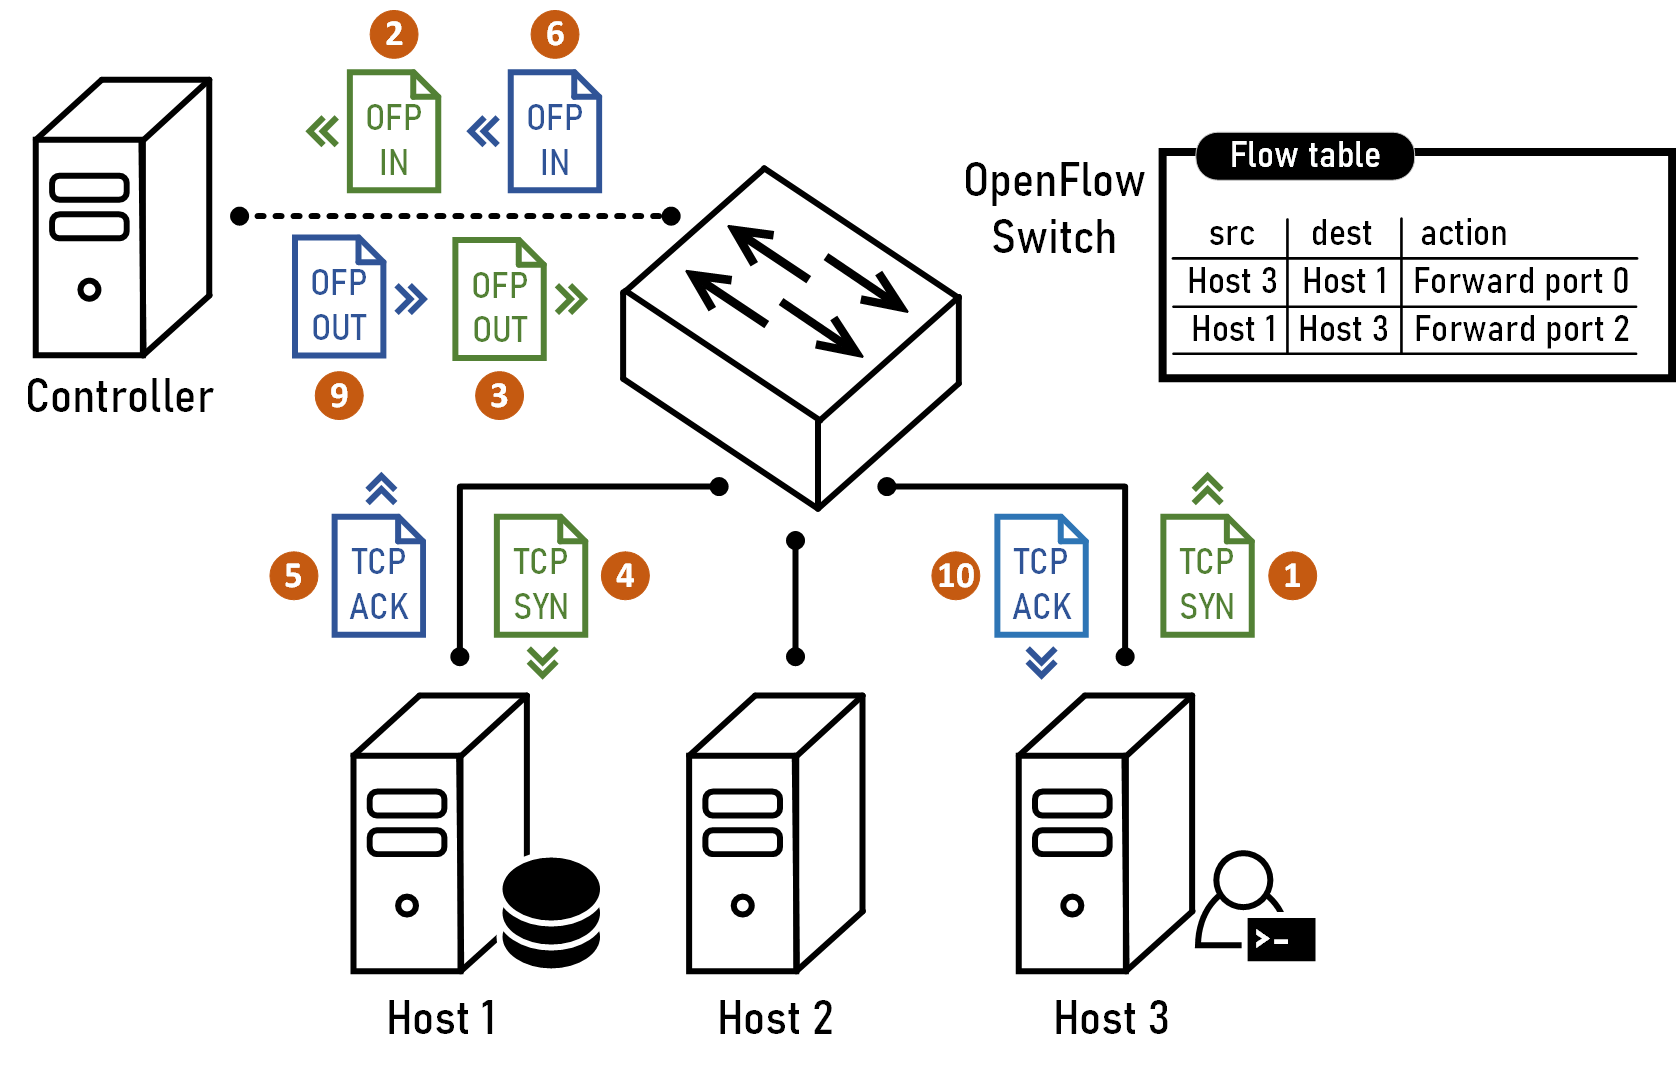
\includegraphics[width=\textwidth]{../Figures/openflow.png}
\caption{An example network with OpenFlow switch. Numbers in the figure 
indicate the order of packets when a user on host 3 connects 
to a server on host 1.}
\label{fig:openflow}
\end{figure}

Figure \ref{fig:openflow} depicts an example of using OpenFlow switch in 
a Local Area Network (LAN). In this figure, \circled{1} a client on Host 3 
sends TCP-SYN packet to OpenFlow switch with the goal of establishing a TCP connection
to a server residing on Host 1. Next, \circled{2} the OpenFlow switch 
cannot find the entry for the flow of this packet. Therefore, it encapsulates 
the packet and forwards it through a secure interface to a controller.
\circled{3} The controller responds to OpenFlow switch using the standardized OpenFlow interface,
and the switch adds a new entry to its flow table. In this case, the flow entry is 
TCP connection packets from host 3 to host 1 with the action of forwarding
packets to port 0.
\circled{4} The switch then forwards TCP-SYN packet to host 1, and \circled{5} 
the server responds to this packet with a TCP-ACK. Again, \circled{6} OpenFlow 
switch has no corresponding flow entry for this packet, and it forwards it to 
controller. \circled{7} With the response of the controller, the switch adds another 
entry to its flow table, and \circled{8} it forwards the packet to the user on host 3.

\subsection{Open Virtual Switch (OVS)}

% explain what is network virtualization function (NVF)